\documentclass[10pt]{article}

\usepackage[a4paper, margin=2.5cm]{geometry}
\usepackage{indentfirst}
\usepackage{fancyhdr}
\usepackage{setspace}
\usepackage{graphicx}
\usepackage{anyfontsize}
\usepackage{amsmath}
\usepackage{tikz}
\usepackage[firstpage=true]{background}
\usetikzlibrary{arrows.meta}

\usepackage[absolute,overlay]{textpos}
\setlength{\TPHorizModule}{1cm}
\setlength{\TPVertModule}{1cm}

\usepackage{xcolor}

\definecolor{myblue}{HTML}{CDE2F7}
\definecolor{myyellow}{HTML}{7297F2}


\pagenumbering{Roman}
\renewcommand{\contentsname}{Contenidos}

\pagestyle{fancy}
		\fancyhf{}
		\fancyfoot[R]{\thepage}
		\fancyfoot[L]{Arquitectura y Tecnología de Redes}
		\fancyhead[C]
		
		
\backgroundsetup{
  scale=1,
  angle=0,
  opacity=0.5,
  contents={
    \begin{tikzpicture}[remember picture, overlay]
      \draw[fill=myyellow] (current page.south west) rectangle (current page.north east);
      \draw[fill=myblue, fill opacity=0.9] (0, 0) rectangle (current page.north east);
      \draw[fill=myblue, fill opacity=1] (current page.south west) rectangle (0, 0);
      \draw[draw=black, line width=0.1cm, fill opacity=1] (0.25, -6.5) rectangle (10.25, -1.75);
    \end{tikzpicture}
  }
}

\begin{document}
	\renewcommand{\footrulewidth}{0.4pt}
	\begin{titlepage}
		\begin{center}
			\vspace*{4cm}		
			\begin{textblock*}{7cm}(2cm, 3cm)   % (width)(x, y) from top-left
    		
\includegraphics[width=7cm]{movistar}
			\end{textblock*}		
			\vspace{11.25cm}
		\end{center}
		
		\begin{textblock*}{8cm} (11cm, 17cm)
			\noindent \fontsize{42}{20} {\textsc{\textbf{PROYECTO \\[0.22cm] DE \\[0.22cm] REDES}}}
		\end{textblock*}
		
		\begin{textblock*}{8cm} (11.25cm, 25cm)
			\Large{\textsc{Lucía Castrillo Sánchez \\[0.1cm] Lucía Cid Varela \\[0.1cm] Héctor Costa Portas \\[0.1cm] Hugo Mera Tato}}	
		\end{textblock*}
	\end{titlepage}
	\newpage
	\tableofcontents
	
	\newpage
	\section{Introducción}
		\indent Este documento esta dedicado al registro de progreso para el proyecto de la asignatura de \\ \textit{Arquitectura y Tecnología de Redes}. La intención es mantener una memoria escrita que informe acerca de todos los procesos realizados para llegar a la maqueta final.
		
	\section{Primer contacto}
	\indent Para empezar, se nos solicita la creación de una maqueta básica en GNS3, que consiste en una estructura con redundancia básica sobre un ISP con tres bucles de abonado.
	\newline \indent Las tareas a completar son:
	\begin{itemize}
		\item Elaboración de la topología básica
		\item Configuración de las IPs necesarias para la conectividad
		\item Implementación de protocolos de red
			\begin{itemize}
				\item DHCP (\textit{Dynamic Host Configuration Protocol})
				\item OSPF (\textit{Open-Shortest Path First})
				\item NAT (\textit{Network Address Translation})
			\end{itemize}
	\end{itemize}
	
	\subsection{Configuración de DHCP}
		\noindent\colorbox{black}{%
    			\parbox{\dimexpr\linewidth-2\fboxsep}{%
        		\color{white}\ttfamily
        		R1\# \\
        		\# \_
    		}%
		}
	\subsection{Configuración de OSPF}
		\noindent\colorbox{black}{%
    			\parbox{\dimexpr\linewidth-2\fboxsep}{%
        		\color{white}\ttfamily
        		R1(config)\# router ospf <ospf\_process\_number> \\
        		R1(config)\# network <interface\_IP> <wildcard> area <area\_number> \\
        		R1(config)\#
    		}%
		} \par \vspace{0.25cm}
		\indent El \textit{wildcard} no es más que el inverso en bits del prefijo de red, es decir, a nivel intuitivo la línea \vspace{0.25cm}\newline
		\noindent\colorbox{black}{%
    			\parbox{\dimexpr\linewidth-2\fboxsep}{%
        		\color{white}\ttfamily
        		10.0.0.0 0.0.0.3	// Esto devuelve las direcciones 10.0.0.0-10.0.0.3
    		}%
		}\vspace{0.25cm} es equivalente a \vspace{0.25cm}\newline
		\noindent\colorbox{black}{%
    			\parbox{\dimexpr\linewidth-2\fboxsep}{%
        		\color{white}\ttfamily
        		10.0.0.0 255.255.255.252	// Esto también devuelve las direcciones 10.0.0.0-10.0.0.3
    		}%
		} \par \vspace{0.25cm} 
		\noindent en cuanto a las direcciones a las que se refieren. \newline
		
		Puede que llame la atención el hecho de que lo que se configure sean las interfaces del router y no el router en sí. Sin embargo, esto tiene sentido práctico, pues permite que escojamos ciertas interfaces para formar parte de un área u otra y así poder segmentar debidamente las redes. Asimismo, facilita la coexistencia de interfaces OSPF con otras de otros IGPs. \newline \par \vspace{0.25cm}
		Para comprobar el correcto funcionamiento de OSPF:  \newline \par \vspace{0.25cm}
		\noindent\colorbox{black}{%
    			\parbox{\dimexpr\linewidth-2\fboxsep}{%
        		\color{white}\ttfamily
        		R1(config)\# show ip ospf neighbor	//Vemos si se ha establecido un vecindario OSPF
        		R1(config)\# show ip route	//Comprobamos que haya rutas creadas por OSPF
    		}%
		}
	\subsection{Configuración de NAT}
\end{document}